\documentclass[11pt,a4paper]{article}
\usepackage[T1]{fontenc}
\usepackage{lmodern}
\usepackage[margin=2.5cm]{geometry}
\usepackage{amsmath,amssymb}
\usepackage{array}
\usepackage{booktabs}
\usepackage{enumitem}
\usepackage{microtype}
\usepackage{placeins}
\usepackage{tikz}
\usetikzlibrary{arrows.meta}
\usepackage[hidelinks]{hyperref}

\newcommand{\code}[1]{\texttt{\detokenize{#1}}}
\newcolumntype{L}[1]{>{\raggedright\arraybackslash}p{#1}}
\setlist{itemsep=2pt,topsep=4pt}
\setlength{\belowcaptionskip}{6pt}
\setlength{\emergencystretch}{4em}

\title{Industry-sector shares in GREU\\ How \code{IndustrySectorsData.jl} builds them}
\author{}
\date{24 November 2026}

\begin{document}
\maketitle

\section{Summary}

The file \code{modules/IndustrySectorsData.jl} builds one data file: \code{industry_sector_shares.csv}.
The file holds the share of each industry that each domestic sector owns, $r_{s,i,t}$.
In the model the name is \code{rIndustrySector_s_i}.

\begin{itemize}
\item There are 63 industries and four domestic sectors: financial corporations, non-financial corporations, government, and households.
\item No source gives the split of an industry over sectors. The file makes a split that agrees with the sector accounts. Its own header calls the shares stylized.
\item The build has four steps. Financial corporations get the finance industries. The government gets shares that match four numbers in the government accounts. Households get shares that match four numbers in the household accounts. Non-financial corporations get the rest.
\item Steps two and three each solve a small optimisation problem. Four targets cannot set 60 shares, so a starting value (the prior) must select the answer.
\item The solve has a defect. It stops before it is at the minimum, and the shares are far from the prior. The government gets 6 per cent of public administration and 90 per cent of employment activities. Section~\ref{sec:defect} shows the cause and a test of two corrections.
\item This note changes no code and no data.
\end{itemize}

All numbers are in EUR million and are for Denmark. They are for 2019 unless the text gives a different year.

\section{Purpose and place in the data build}

An industry groups producers by what they make. A sector groups units by who controls them.
The input-output accounts are by industry. The sector accounts are by sector.
The model needs both: it makes output, wages, and capital by industry, and it has a budget for each sector.
The shares $r_{s,i,t}$ are the link.

Three files use the shares.
\begin{itemize}
\item \code{modules/IndustrySectors.jl} reads the file. A sector gets the share $r_{s,i,t}$ of the output, the intermediate inputs, the wages, the production taxes, the capital, the investment, and the persons of each industry. The shares are constant after the calibration year.
\item \code{modules/TaxesData.jl} reads the file when it splits other production taxes over industries. The part of an industry that the government owns has a weight of zero in the tax base.
\item \code{RefreshData.jl} runs the build. The section comes after the input-output, production, sector-account, and government data. It also comes after the step in \code{TaxesData.jl} that reconciles net production taxes, and before the step that writes the tax tables.
\end{itemize}

The file is also a script. This command runs the build and writes the file:
\begin{verbatim}
julia --project=. model_julia/modules/IndustrySectorsData.jl
\end{verbatim}

\section{Inputs}

Table~\ref{tab:inputs} shows the source files. They are in \code{model_julia/data}. The build reads them with \code{read_cells} and downloads nothing.

\begin{table}[!htbp]
\centering
\footnotesize
\caption{Input files. The headings in italics are the folders}
\label{tab:inputs}
\begin{tabular}{@{}L{5.5cm}L{5.0cm}L{4.4cm}@{}}
\toprule
File & Variable & Content \\
\midrule
\multicolumn{3}{@{}l}{\textit{input\_output}} \\
\code{input_output_supply.csv} & \code{qY_p_i} & Output by product and industry \\
\code{input_output_purchaser_use.csv} & \code{qPurchaserUse_p_u} & Use by product and user \\
\code{input_output_margins.csv} & \code{qMarginBundle_p_u} & Trade and transport margins \\
\code{input_output_net_product_tax.csv} & \code{vntProduct_p_u} & Net product taxes \\
\addlinespace
\multicolumn{3}{@{}l}{\textit{production}} \\
\code{production_labor.csv} & \code{vWages_i} & Wages by industry \\
\code{production_gva.csv} & \code{vntProduction_i} & Other production taxes less subsidies by industry \\
\addlinespace
\multicolumn{3}{@{}l}{\textit{government}} \\
\code{government_variables.csv} & \code{vGovIntermediateCons} \newline \code{vGovEmplComp} \newline \code{vtGovProductionPaidSource} \newline \code{vsGovProductionReceivedSource} & Government targets \\
\addlinespace
\multicolumn{3}{@{}l}{\textit{sector\_accounts}} \\
\code{non_financial_transactions.csv} & \code{NonFinancialTransactions} & Household targets \\
\code{sector_accounts.csv} & \code{vGrossOpSurplusMixedIncome} & Operating surplus and mixed income by sector \\
\bottomrule
\end{tabular}
\end{table}

\paragraph{Industries and years.}
The industries are those with output in the calibration year, 2019. There are 63.
The build makes shares for the year before the calibration year and for the calibration year, if all targets exist. The file now has 2018 and 2019.

\paragraph{Industry groups.}
The function \code{industries_in_sections} gives three groups from the NACE sections.
\begin{itemize}
\item \code{financial_industries}: section K. These are K64, K65, and K66.
\item \code{government_core_industries}: sections O, P, and Q. These are O, P, Q86, and Q87--88.
\item \code{household_housing_industries}: section L. This is the one industry L.
\end{itemize}

\section{Industry accounts}

The function \code{industry_accounts} makes a production account for each industry $i$ and year.
It uses the same cells as the model, so the model gets the same totals.
\begin{align*}
Y_i &= \text{output at basic prices}, \\
M_i &= \text{use} + \text{margins} + \text{net product taxes} \quad \text{(intermediate inputs at purchaser prices)}, \\
W_i &= \text{wages}, \\
N_i &= \text{other production taxes less subsidies}, \\
C_i &= M_i + W_i + N_i \quad \text{(operating cost)}, \\
B_i &= Y_i - C_i \quad \text{(gross operating surplus)}.
\end{align*}
Table~\ref{tab:accounts} shows the accounts of the three industry groups.

\begin{table}[!htbp]
\centering
\small
\caption{Industry accounts, 2019. EUR million}
\label{tab:accounts}
\begin{tabular}{@{}lrrrrrr@{}}
\toprule
 & Output & Intermediate & Wages & Production & Operating & Operating \\
 & & inputs & & taxes, net & cost & surplus \\
 & $Y$ & $M$ & $W$ & $N$ & $C$ & $B$ \\
\midrule
Finance (K64, K65, K66) & 26,088 & 11,649 & 7,604 & 1,122 & 20,374 & 5,714 \\
Public (O, P, Q86, Q87--88) & 82,277 & 25,393 & 49,532 & 89 & 75,014 & 7,263 \\
Real estate (L) & 41,911 & 12,083 & 2,283 & 2,667 & 17,033 & 24,878 \\
Other 55 industries & 397,651 & 230,251 & 100,436 & $-578$ & 330,109 & 67,542 \\
\midrule
All 63 industries & 547,927 & 279,376 & 159,855 & 3,300 & 442,530 & 105,397 \\
\bottomrule
\end{tabular}
\end{table}

\section{Sector targets}

Each sector has a target for gross operating surplus. For households the target includes mixed income.
The government and the households also have targets for the three cost items.
Table~\ref{tab:targets} shows the targets and their sources.

\begin{table}[!htbp]
\centering
\small
\caption{Sector targets, 2019. EUR million}
\label{tab:targets}
\begin{tabular}{@{}lrrrr@{}}
\toprule
 & Financial & Non-financial & Government & Households \\
 & corporations & corporations & & \\
\midrule
Intermediate inputs, $\bar M_s$ & & & 26,397 & 21,453 \\
Wages, $\bar W_s$ & & & 46,691 & 8,494 \\
Production taxes, net, $\bar N_s$ & & & $-53$ & 1,473 \\
Operating cost, $\bar C_s$ & & & 73,035 & 31,420 \\
Operating surplus, $\bar B_s$ & 5,621 & 68,871 & 8,121 & 22,783 \\
\bottomrule
\end{tabular}
\end{table}

\begin{itemize}
\item \textbf{Operating surplus} is \code{vGrossOpSurplusMixedIncome} from the sector accounts, for all four sectors. The four targets add to 105,396. The industry accounts give 105,397.
\item \textbf{Government costs} are from the government accounts: intermediate consumption, employee compensation, and other production taxes paid less subsidies received.
\item \textbf{Household costs} are from the non-financial transactions of the household sector: P.2 paid, D.1 paid, and D.29 paid less D.39 received.
\item \textbf{Operating cost} is the sum of the three cost items.
\end{itemize}

\section{The four steps}

The function \code{stylized_shares} makes the shares of one year. Figure~\ref{fig:steps} shows the order.
The order matters: each step takes what the steps before it left.

\begin{figure}[!htbp]
\centering
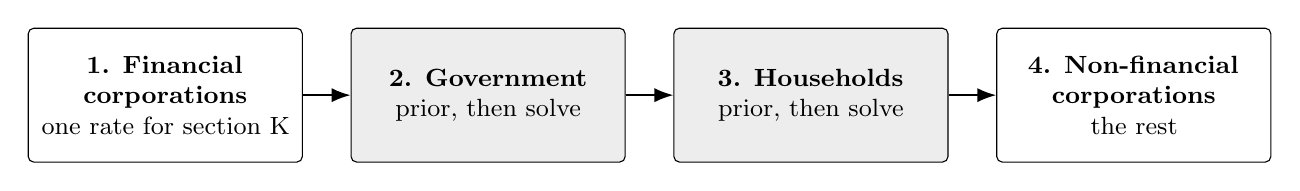
\begin{tikzpicture}[
  font=\small,
  box/.style={draw, rounded corners=2pt, align=center, inner sep=4pt, minimum height=17mm, text width=32mm},
  flow/.style={-{Latex[length=2.4mm]}, line width=0.6pt},
]
\node[box] (f) at (0,0) {\textbf{1. Financial corporations}\\ one rate for section K};
\node[box, fill=black!7] (g) at (4.1,0) {\textbf{2. Government}\\ prior, then solve};
\node[box, fill=black!7] (h) at (8.2,0) {\textbf{3. Households}\\ prior, then solve};
\node[box] (n) at (12.3,0) {\textbf{4. Non-financial corporations}\\ the rest};
\draw[flow] (f) -- (g);
\draw[flow] (g) -- (h);
\draw[flow] (h) -- (n);
\end{tikzpicture}
\caption{The steps in \code{stylized_shares}. The grey steps solve an optimisation problem.}
\label{fig:steps}
\end{figure}

\subsection{Step 1: financial corporations}

Financial corporations get the same share of each finance industry and nothing of the other industries.
The share is the surplus target divided by the surplus of the finance industries:
\[
r_{F,i} = \frac{\bar B_F}{\sum_{j \in K} B_j} = \frac{5{,}621}{5{,}714} = 0.984 \quad \text{for } i \in K .
\]
Government and households get nothing of the finance industries, so non-financial corporations get the other 0.016.

\subsection{Step 2: government}

\paragraph{Prior.}
The function \code{government_prior} sets a starting value for each industry.
\begin{itemize}
\item If the surplus target is below the surplus of the public industries, the public industries get the share target divided by surplus, and the other industries get zero.
\item If not, the public industries get a share of one. The other industries, without finance, get one equal share that fills the gap.
\end{itemize}
In 2019 the target is 8,121 and the surplus of the public industries is 7,263. The prior is then 1.000 for O, P, Q86, and Q87--88, zero for finance, and $858 / 92{,}420 = 0.0093$ for the other 56 industries.
The prior matches the surplus target. It does not match the cost targets: it gives wages of 50,485 and the target is 46,691.

\paragraph{Solve.}
The function \code{target_shares} changes the prior so that the shares match the government targets. Section~\ref{sec:problem} gives the problem.
The upper limit of a share is one, and zero for the finance industries.

\subsection{Step 3: households}

\paragraph{Prior.}
The function \code{household_prior} uses two numbers from the household accounts: operating surplus (B.2g, 11,396), which is from dwellings, and mixed income (B.3g, 11,230).
\begin{itemize}
\item Real estate (L) gets the share operating surplus divided by its industry surplus: $11{,}396 / 24{,}878 = 0.458$.
\item Finance gets zero.
\item All other industries get one equal share, mixed income divided by their surplus: $11{,}230 / 74{,}805 = 0.150$.
\end{itemize}

\paragraph{Solve.}
The same function \code{target_shares} changes the prior to match the household targets.
The upper limit of a share is what the first two steps left: $1 - r_{F,i} - r_{G,i}$.

\subsection{Step 4: non-financial corporations}

Non-financial corporations get the rest of each industry:
\[
r_{N,i} = 1 - r_{F,i} - r_{G,i} - r_{H,i} .
\]
This sector has no cost targets. Its surplus target holds because the four surplus targets add to the industry total.

\section{The optimisation problem}
\label{sec:problem}

The function \code{target_shares} solves this problem for one sector $s$ and one year.
The unknowns are the shares $r_i$ of the 63 industries. The prior is $r^0_i$, and $c_i$ is the upper limit.
\begin{align}
\min_{r} \quad & \sum_{X \in \{M, W, N\}} \left( \frac{\sum_i r_i X_i - \bar X_s}{\bar X_s} \right)^{2}
 + \omega \sum_i \left( r_i - r^0_i \right)^2 \label{eq:objective} \\
\text{subject to} \quad & \sum_i r_i C_i = \bar C_s , \label{eq:cost} \\
 & \sum_i r_i B_i = \bar B_s , \label{eq:surplus} \\
 & 0 \le r_i \le c_i . \nonumber
\end{align}
The weight is $\omega = 10^{-8}$.

\begin{itemize}
\item \textbf{Two targets are constraints.} Operating cost (\ref{eq:cost}) and operating surplus (\ref{eq:surplus}) must hold exactly. In the code they are \code{sector_target_component}.
\item \textbf{Three targets are in the objective.} The first term is the squared relative error of intermediate inputs, wages, and production taxes. In the code they are \code{source_component}. Their sum is operating cost, so only two of the three are free.
\item \textbf{The prior is in the objective with a small weight.} The second term is the squared distance to the prior.
\item \textbf{The solver is Ipopt.} It starts at the prior. The option \code{bound_relax_factor} is zero, so a share cannot go below zero or above its limit.
\end{itemize}

The problem has four independent targets and 60 free shares. Many sets of shares match all four targets, and for all of them the first term is zero.
The correct answer is the set that is nearest to the prior. For this answer the size of $\omega$ does not matter, if it is small.
The purpose of the small weight is clear: match the targets first, then stay near the prior.

\section{Checks and output}

After the solve, \code{stylized_shares} makes these checks. A failure stops the build.
\begin{itemize}
\item Each share is from zero to one.
\item The four shares of an industry add to one.
\item Each sector gets its surplus target. The tolerance is 2.0, for rounding in the sources.
\item Government and households get their cost target and their surplus target, with the same tolerance.
\end{itemize}
The checks do not include the three cost items and the distance to the prior.

\code{refresh_industry_sector_shares!} writes the file. The file has one row for each sector, industry, and year: 504 rows.
It has four columns. The first three are \code{variable}, \code{indices}, and \code{value}. The last is \code{assumption}: one sentence on the rule for that share.

\section{Results}

Table~\ref{tab:sectors} shows the sector accounts that the shares in the file give. All targets hold.

\begin{table}[!htbp]
\centering
\small
\caption{Sector accounts from the shares in the file, 2019. EUR million}
\label{tab:sectors}
\setlength{\tabcolsep}{5pt}
\begin{tabular}{@{}lrrrrrr@{}}
\toprule
 & Output & Intermediate & Wages & Production & Operating & Industries \\
 & & inputs & & taxes, net & surplus & with a share \\
\midrule
Financial corporations & 25,663 & 11,458 & 7,480 & 1,103 & 5,621 & 3 \\
Non-financial corporations & 386,906 & 220,067 & 97,190 & 777 & 68,872 & 63 \\
Government & 81,156 & 26,397 & 46,691 & $-53$ & 8,121 & 60 \\
Households & 54,203 & 21,453 & 8,494 & 1,473 & 22,783 & 60 \\
\midrule
All & 547,927 & 279,376 & 159,855 & 3,300 & 105,397 & \\
\bottomrule
\end{tabular}
\end{table}

Table~\ref{tab:shares} shows the shares of some industries. Some of them are not credible.
The government owns 6 per cent of public administration, 90 per cent of employment activities, and 84 per cent of households as employers.
Households own 48 per cent of the pharmaceutical industry.

\begin{table}[!htbp]
\centering
\small
\caption{Shares in the file for some industries, 2019}
\label{tab:shares}
\begin{tabular}{@{}llrrrr@{}}
\toprule
Industry & & Financial & Non-financial & Government & Households \\
 & & corporations & corporations & & \\
\midrule
K64 & Financial services & 0.984 & 0.016 & 0.000 & 0.000 \\
L & Real estate & 0.000 & 0.432 & 0.003 & 0.565 \\
O & Public administration & 0.000 & 0.920 & 0.060 & 0.020 \\
P & Education & 0.000 & 0.007 & 0.987 & 0.006 \\
Q86 & Health & 0.000 & 0.067 & 0.916 & 0.017 \\
Q87--88 & Social work & 0.000 & 0.010 & 0.983 & 0.007 \\
N78 & Employment activities & 0.000 & 0.057 & 0.905 & 0.038 \\
T & Households as employers & 0.000 & 0.086 & 0.836 & 0.078 \\
G47 & Retail trade & 0.000 & 0.743 & 0.223 & 0.035 \\
C21 & Pharmaceuticals & 0.000 & 0.499 & 0.021 & 0.480 \\
A01 & Agriculture & 0.000 & 0.860 & 0.077 & 0.062 \\
\bottomrule
\end{tabular}
\end{table}

\FloatBarrier
\section{A defect: the solve stops before the minimum}
\label{sec:defect}

\subsection{Cause}

The shares in the file match the targets, but they are not the solution of problem (\ref{eq:objective}).
The government shares in the file have a squared distance to the prior of 2.97. The lowest distance that matches the same targets is 0.045.

The cause is the size of the weight. The prior term in (\ref{eq:objective}) is of the order $10^{-8}$.
The default tolerance of Ipopt is also $10^{-8}$. When the shares match the targets, the error that Ipopt measures is below its tolerance, and it stops.
The prior term then has no effect. The answer is where the steps of the solver ended, and this has no economic meaning.

\subsection{Test}

A test for this note solved the same problem with the same data in three ways.
\begin{itemize}
\item \textbf{Code now.} Weight $10^{-8}$ and the default tolerance. This gives the shares in the file.
\item \textbf{Low tolerance.} Weight $10^{-8}$ and the Ipopt option \code{tol} at $10^{-13}$.
\item \textbf{Targets as constraints.} All four targets ($M$, $W$, $N$, $B$) are constraints. The objective is only the distance to the prior, with no weight.
\end{itemize}
Table~\ref{tab:test} shows the result. In all three rows the government and the households match all their targets.
The last two rows agree with each other, and they are the true minimum.

\begin{table}[!htbp]
\centering
\small
\caption{Test of the solve, 2019}
\label{tab:test}
\setlength{\tabcolsep}{4.5pt}
\begin{tabular}{@{}lrrrrrrrrr@{}}
\toprule
 & \multicolumn{5}{c}{Government share} & \multicolumn{2}{c}{Distance to prior} & Household & Government \\
\cmidrule(lr){2-6}\cmidrule(lr){7-8}
 & O & P & Q86 & Q87--88 & N78 & Gov. & Hh. & share of L & output from \\
 & & & & & & & & & O, P, Q \\
\midrule
Code now & 0.060 & 0.987 & 0.916 & 0.983 & 0.905 & 2.970 & 0.665 & 0.565 & 59,602 \\
Low tolerance & 0.938 & 0.934 & 0.908 & 0.935 & 0.000 & 0.045 & 0.361 & 0.618 & 76,429 \\
Constraints & 0.939 & 0.935 & 0.909 & 0.935 & 0.000 & 0.045 & 0.361 & 0.618 & 76,466 \\
\bottomrule
\end{tabular}
\end{table}

\begin{itemize}
\item With a correct solve the government owns 91 to 94 per cent of each public industry. The public industries then give 94 per cent of government output. They give 73 per cent with the shares in the file.
\item The shares cannot be one. Wages in the public industries are 49,532 and the wage target is 46,691.
\item The household shares have the same defect. The largest change in a household share is 0.23. The largest change in a government share is 0.90.
\item The year 2018 has the same defect. The government share of public administration is 0.056 in the file and 0.947 with a correct solve.
\end{itemize}

\subsection{Effects in the model}

The sector totals of the calibration year match the sources with all three sets of shares. The defect changes what is behind the totals.
\begin{itemize}
\item \textbf{Responses to shocks.} The government sector follows employment activities, retail trade, and other private industries. It follows public administration very little.
\item \textbf{Persons and capital by sector.} The model uses the same shares for persons, capital, and investment.
\item \textbf{Corporation tax.} Non-financial corporations get 92 per cent of public administration. This puts its operating surplus in their taxable income, and it gives the industry a marginal corporation tax rate.
\item \textbf{Other production taxes.} \code{TaxesData.jl} gives the government part of an industry a weight of zero in the tax base. With a share of 6 per cent, public administration has almost its full weight.
\end{itemize}
The note \code{public_sector.tex} gives the numbers for the government sector.

\subsection{Possible corrections}

The test shows two corrections that give the same shares.
\begin{enumerate}
\item Make the four targets constraints and minimise only the distance to the prior. This has no weight to select, and the result does not depend on the tolerance. The cost constraint (\ref{eq:cost}) is then not necessary.
\item Keep the problem and set a lower tolerance.
\end{enumerate}
After a correction, run the build again and then the sections after it in \code{RefreshData.jl}. Then run \code{Calibrate.jl}.
The test changed no file in the repository.

\section{Limits of the method}

These limits stay after a correction of the solve.
\begin{itemize}
\item \textbf{The split is an assumption.} The sources give no data on sectors by industry. Four targets for each sector set the totals and not the split. The prior sets the split.
\item \textbf{One share for all accounts.} A sector gets the same share of output, inputs, wages, taxes, and surplus of an industry. A government unit and a private unit in the same industry then have the same cost structure.
\item \textbf{The household prior is far from the household targets.} The prior of 0.150 in all industries gives intermediate inputs of 43,913 and wages of 23,560. The targets are 21,453 and 8,494. The solve must change the shares much, and the result has high household shares in some industries, such as pharmaceuticals.
\item \textbf{The household prior can be above the limit.} In education the limit for households is 0.013 after the government step. The prior is 0.150.
\item \textbf{The order of the steps matters.} The government takes its shares before the households.
\item \textbf{The error of production taxes is relative to a small target.} The government target is $-53$, so a small error in level is a large relative error.
\item \textbf{Shares are for two years.} The model keeps the shares of 2019 constant in all later years.
\end{itemize}

The numbers in this note are from the data files and the code of 24 November 2026. The scripts that made the tables and the test are not in the repository.

\end{document}
